\def\year{2019}\relax
\documentclass[letterpaper]{article} % DO NOT CHANGE THIS
\usepackage{aaai19}  % DO NOT CHANGE THIS
\usepackage{times}  % DO NOT CHANGE THIS
\usepackage{helvet} % DO NOT CHANGE THIS
\usepackage{courier}  % DO NOT CHANGE THIS
\usepackage[hyphens]{url}  % DO NOT CHANGE THIS
\usepackage{graphicx} % DO NOT CHANGE THIS
\urlstyle{rm} % DO NOT CHANGE THIS
\def\UrlFont{\rm}  % DO NOT CHANGE THIS
\usepackage{graphicx}  % DO NOT CHANGE THIS
\frenchspacing  % DO NOT CHANGE THIS
\setlength{\pdfpagewidth}{8.5in}  % DO NOT CHANGE THIS
\setlength{\pdfpageheight}{11in}  % DO NOT CHANGE THIS
\nocopyright
\graphicspath{{images/}}
\usepackage{array}
\usepackage{amsmath}
\usepackage{caption}
%PDF Info Is REQUIRED.
% For /Author, add all authors within the parentheses, separated by commas. No accents or commands.
% For /Title, add Title in Mixed Case. No accents or commands. Retain the parentheses.
\pdfinfo{
/Title (Image Enhancement Applied to Dynamic Frame Generation)
/Author (Mark Wesley Harris)
} %Leave this	
% /Title ()
% Put your actual complete title (no codes, scripts, shortcuts, or LaTeX commands) within the parentheses in mixed case
% Leave the space between \Title and the beginning parenthesis alone
% /Author ()
% Put your actual complete list of authors (no codes, scripts, shortcuts, or LaTeX commands) within the parentheses in mixed case. 
% Each author should be only by a comma. If the name contains accents, remove them. If there are any LaTeX commands, 
% remove them. 

% DISALLOWED PACKAGES
% \usepackage{authblk} -- This package is specifically forbidden
% \usepackage{balance} -- This package is specifically forbidden
% \usepackage{caption} -- This package is specifically forbidden
% \usepackage{color (if used in text)
% \usepackage{CJK} -- This package is specifically forbidden
% \usepackage{float} -- This package is specifically forbidden
% \usepackage{flushend} -- This package is specifically forbidden
% \usepackage{fontenc} -- This package is specifically forbidden
% \usepackage{fullpage} -- This package is specifically forbidden
% \usepackage{geometry} -- This package is specifically forbidden
% \usepackage{grffile} -- This package is specifically forbidden
% \usepackage{hyperref} -- This package is specifically forbidden
% \usepackage{navigator} -- This package is specifically forbidden
% (or any other package that embeds links such as navigator or hyperref)
% \indentfirst} -- This package is specifically forbidden
% \layout} -- This package is specifically forbidden
% \multicol} -- This package is specifically forbidden
% \nameref} -- This package is specifically forbidden
% \natbib} -- This package is specifically forbidden -- use the following workaround:
% \usepackage{savetrees} -- This package is specifically forbidden
% \usepackage{setspace} -- This package is specifically forbidden
% \usepackage{stfloats} -- This package is specifically forbidden
% \usepackage{tabu} -- This package is specifically forbidden
% \usepackage{titlesec} -- This package is specifically forbidden
% \usepackage{tocbibind} -- This package is specifically forbidden
% \usepackage{ulem} -- This package is specifically forbidden
% \usepackage{wrapfig} -- This package is specifically forbidden
% DISALLOWED COMMANDS
% \nocopyright -- Your paper will not be published if you use this command
% \addtolength -- This command may not be used
% \balance -- This command may not be used
% \baselinestretch -- Your paper will not be published if you use this command
% \clearpage -- No page breaks of any kind may be used for the final version of your paper
% \columnsep -- This command may not be used
% \newpage -- No page breaks of any kind may be used for the final version of your paper
% \pagebreak -- No page breaks of any kind may be used for the final version of your paperr
% \pagestyle -- This command may not be used
% \tiny -- This is not an acceptable font size.
% \vspace{- -- No negative value may be used in proximity of a caption, figure, table, section, subsection, subsubsection, or reference
% \vskip{- -- No negative value may be used to alter spacing above or below a caption, figure, table, section, subsection, subsubsection, or reference

\setcounter{secnumdepth}{0} %May be changed to 1 or 2 if section numbers are desired.

% The file aaai19.sty is the style file for AAAI Press 
% proceedings, working notes, and technical reports.
%
\setlength\titlebox{2.5in} % If your paper contains an overfull \vbox too high warning at the beginning of the document, use this
% command to correct it. You may not alter the value below 2.5 in
\title{Image Enhancement Applied to Dynamic Frame Generation}
%Your title must be in mixed case, not sentence case. 
% That means all verbs (including short verbs like be, is, using,and go), 
% nouns, adverbs, adjectives should be capitalized, including both words in hyphenated terms, while
% articles, conjunctions, and prepositions are lower case unless they
% directly follow a colon or long dash
\author{Mark Wesley Harris\\ % All authors must be in the same font size and format. Use \Large and \textbf to achieve this result when breaking a line
% If you have multiple authors and multiple affiliations
% use superscripts in text and roman font to identify them. For example, Sunil Issar,\textsuperscript{\rm 2} J. Scott Penberthy\textsuperscript{\rm 3} George Ferguson,\textsuperscript{\rm 4} Hans Guesgen\textsuperscript{\rm 5}. Note that the comma should be placed BEFORE the superscript for optimum readability
University of Colorado Colorado Springs\\
wharris2@uccs.edu % email address must be in roman text type, not monospace or sans serif
\And
Jugal Kalita\\
University of Colorado Colorado Springs\\
jkalita@uccs.edu
}
\begin{document}

\maketitle

\begin{abstract}
Image processing is
widely studied in Computer Graphics, and
%a growing topic of interest within the Computer Graphics community.
image enhancement in particular is growing in popularity.
Our goal is to find the architecture best suited for
enhancing images by removing
noise and other visual artifacts from an input image.
Of those researched in the past decade,
there are a few architectures that regularly perform better for this task than others.
Here we discuss our evaluation of two of these models,
Generative Adversarial Networks and Transformers.
\end{abstract}

\section{Introduction}
Enhancing images cannot be accomplished realistically with tradition means,
so researchers are now turning to machine learning to solve
this and other complex image processing problems.
Image enhancement involves not only increasing image resolution
(called super-resolution), but also replacing noise and other anomalies with
believable substitutes.
Here we discuss our progress in evaluating
the DCGAN, SRGAN, and Transformer architectures
applied to image enhancement.
We hope the conclusion of this research will
provide a foundation
future advancements in image processing
and Computer Graphics research.

\section{Related Work}
Here we discuss foundational concepts related to this project.
Our code and evaluations were based off of the DCGAN
\cite{generative_adversarial_networks}, SRGAN
\cite{srgan}, and Sparse Attention
\cite{generative_transformers} research papers.

\subsection{Generative Adversarial Network}
The Generative Adversarial Network (GAN)
was first proposed as a way to train a model to produce more realistic images.
The network is made up of two architectures:
a generator, G, and a discriminator, D.
GAN's are able to generate new images that have similar qualities to
those in the dataset which they are trained on
\cite{generative_adversarial_networks}.

\begin{figure}[htbp]
\centerline{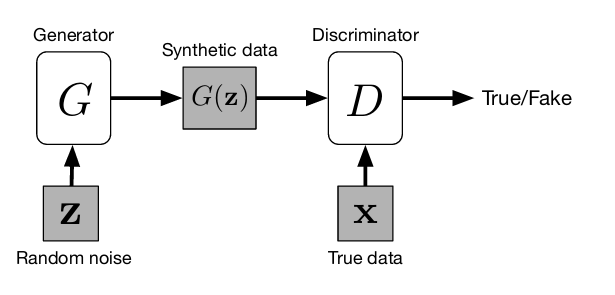
\includegraphics[width=7cm]{gan_architecture.png}}
\caption{Basic Generative Adversarial Network architecture, with a generator $G$
and discriminator $D$
\cite{cgan}.}
\label{fig:gan_architecture}
\end{figure}

The generalized GAN architecture is shown in Figure \ref{fig:gan_architecture}.
The model works by training both the generator $G$ and
discriminator $D$ in tandem.
$G$ is trained to progressively generate more realistic images,
while $D$ is trained to recognize differences between real and fake inputs.
This relationship can be expressed in the format of a
``two-player min-max game'', shown in Equation \ref{eq:gan_basic}.
Here, $p_{data}(\mathbf{x})$ represents the true data distribution,
and $p_{z}(\mathbf{z})$ represents the distribution of noise.
The goal in training a GAN is to minimize error in the generator
and maximize error detection in the discriminator \cite{cgan}.
Optimizations and variants can be made from this simple concept, of which include
the implementations of cGAN, DCGAN, and SRGAN.

\begin{equation}
\label{eq:gan_basic}
\begin{split}
\text{min}_G\text{max}_DV(D,G) &=
E_{\mathbf{x}\sim p_{data}(\mathbf{x})}[\log D(\mathbf{x})] \\
&+ E_{\mathbf{z}\sim p_{z}(\mathbf{z})}[\log(1 - D(G(\mathbf{z})))]
\end{split}
\end{equation}

\subsection{Transformer}
The Transformer was first proposed
as a way to use attention mechanisms more efficiently.
The architecture relies
``\dots entirely on self-attention to compute representations of its input and output
without using sequence-aligned RNNs or convolution''
\cite{attention_need}.
The Encoder and Decoder for the Transformer design
are shown in Figure \ref{fig:attention}.
An input is first encoded into the dimensional space
the transformer works with.
Then the transformed data is processed
and decoded back into a conceivable output.

\begin{figure}[htbp]
\centerline{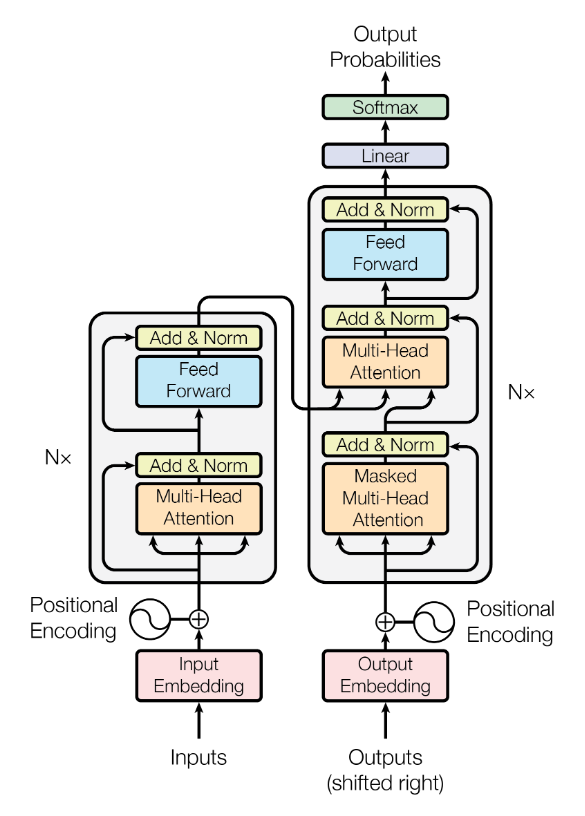
\includegraphics[width=6cm]{attention_architecture.png}}
\caption{Transformer architecture
\cite{attention_need}.}
\label{fig:attention}
\end{figure}

%The Transformer uses a series of attention functions to map
%between two sequences.
%An attention function is
%``\dots mapping [of] a query and a
%set of key-value pairs to an output''
%\cite{attention_need}.
%The mathematical expression of an attention function is shown in
%Equation \ref{eq:attention}.
%$d_k$ is the dimension of keys and queries, and
%$Q,K,V$ are matrices of queries, keys, and values, respectively.
%The function uses dotproduct, so that the output is computed as
%a weighted sum of the values
%\cite{attention_need}.
%
%\begin{equation}
%\label{eq:attention}
%\begin{split}
%\text{Attention}(Q,K,V) = \text{softmax}(\frac{QK^T}{\sqrt{d_k}})V
%\end{split}
%\end{equation}

Transformers are able to
``\dots model arbitrary dependencies
in a constant number of layers,''
and have proven useful for natural language processing and image generation
\cite{generative_transformers}.
The focus of the model is to find what parts of a sequence are relevant to other parts,
in order to make generalizations and extrapolate from the data.
We can model the joint probability of a sequence,
$\mathbf{x}={x_1,x_2,\dots,x_n}$,
as the product of conditional
probability distributions and parameterized by a network $\theta$
\cite{generative_transformers}.
The final expression is shown in Equation \ref{eq:attention_prob}.

\begin{equation}
\label{eq:attention_prob}
p(\mathbf{x}) = \prod_{i=1}^{n}p(x_i|x_1,\dots,x_{i-1};\theta)
\end{equation}


The Transformer is a recent concept that still has many inherent problems.
One of the major problems with the architecture
is that the resources it requires scales with $O(n^2)$,
for sequence length $n$. However, it is theorized that
``\dots to improve computational performance for tasks involving very long sequences,
self-attention could be restricted to considering only a neighborhood of size $r$''
\cite{attention_need}.

The Sparse Transformer architecture was developed as a means to shrink the
growth of computational resources for large sequences.
This variant introduced sparse factorizations on the attention matrix
of a Transformer in order to speed up processing.
An approximation of the dense attention
operation is found by combining several cheaper attention operations.
The result was a faster attention-based architecture
that could be trained on longer sequences of data.
Figure \ref{fig:attention_optimization} shows a visual representation of
the two optimizations experimented with, strided and fixed.

\begin{figure}[htbp]
\centerline{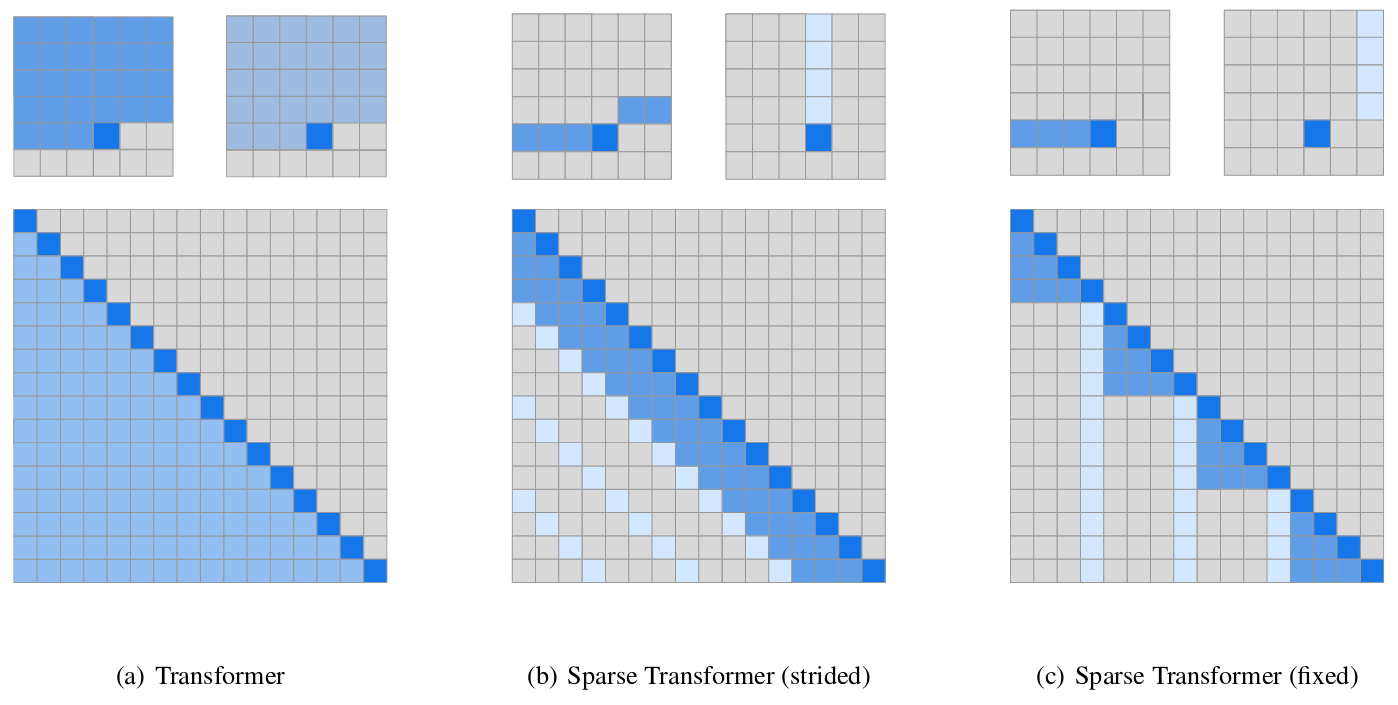
\includegraphics[width=7cm]{attention_comparison.png}}
\caption{Optimizations of Attention
\cite{generative_transformers}.}
\label{fig:attention_optimization}
\end{figure}

The Sparse Transformer architecture reduces the resource cost to
$O(n\sqrt[p]{n})$.
The architecture is also simpler than other autoregressive models that perform
similar functions, including upscaling and enhancement \cite{pixel_subscale}.

\section{Approach}
The source code for each model was copied and modified accordingly
during development.
The DCGAN and SRGAN implementations were written for PyTorch,
while the Transformer architecture used TensorFlow.
A python module of utility functions was created and shared between the models,
so that evaluations of altered images would be consistent.
A dataset of approximately 14,000 32 x 32 pixel images was created
for the purposes of training and testing the developed networks.
It is also planned that the CIFAR dataset will be used later to provide
further benchmarking.

Equation \ref{eq:alter} expresses how images were degraded to provide the sources for enhancement.
First, a random sample of uniform noise, $I^{N}$, was generated in the shape of
sample image, $I$. A linear combination was applied to add $\alpha$ amount of the input
image with $1 - \alpha$ amount of the random noise
(where $0 \leq \alpha \leq 1$).
Afterwards, a Gaussian blur was applied with scale $\beta$.
Figure \ref{fig:srgan_outputs} shows altered samples
of an image from the dataset with varying parameters of $\alpha$ and $\beta$.

\begin{equation}
\label{eq:alter}
I' = G_{\beta,\beta}(\alpha I + (1 - \alpha)I^{N})
\end{equation}

\subsection{Methods}
The first approach studied was the
Deep Convolutional GAN (DCGAN).
The DCGAN
is similar to the GAN,
but uses convolutional and convolutional-transpose layers in D and G, respectively
\cite{unsupervised_learning}.
The Pose Guided Person Image Generation (PG\textsuperscript{2}) system
proved that a variant conditional DCGAN could be used to
remove anomalies and provide higher resolution for images
\cite{pose_guided_image_generation}.

The second approach studied was the
Super Resolution GAN (SRGAN).
The SRGAN was first developed in
Single Image Super Resolution (SISR) research, and showed a drastic decrease in loss measurements
compared to ``NN, bicubic interpolation, and four state-of-the-art methods''
\cite{srgan}.

The third architecture looked at was the Transformer,
taken from the Sparse Attention project \cite{generative_transformers}.
There were problems early on with running the base model, however,
so testing for this architecture was rescheduled for a later milestone.

\subsection{Challenges}
Since the base DCGAN architecture was created for image generation from noise,
there was no way to inject a conditioning image during training.
Several methods were attempted to fix this problem.
We first attempted to manipulate the Z-latent vector
(the vector that the GAN trains in each epoch).
Each of the 100 elements of the vector maps features of one image to another.
Since the latent vector is unknown until training occurs,
it was impractical to initialize it without a way to convert
the condition image into the latent space.
After several attempts, this method was abandoned.

The next approach proved to be more useful than manipulating the latent vector.
The model was made to generate $G(\mathbf{x})$ of
the expression $I_E = X - G(\mathbf{x})$. The theory behind this approach is that
the model would learn to generate the enhanced image through
the inverse of noise and other alterations the image was subjected to.
%However, with the way the generator is setup, back-propagation acts on the image generated
%and not the calculated image, $I_E$.
%Thus, the generator became quickly confused.
This was the method employed for evaluation of the DCGAN,
however further experimentation is planned to create a model
that works as expected.

\subsection{Evaluation}
One major criticism for GAN's is the
``lack of a robust and consistent evaluation method\dots''
\cite{gmm}.
There is no objective function optimized in a GAN,
and GAN's operate on a learned latent space
which cannot be evaluated tangibly.
Thus, in order to evaluate the GAN models,
%we must work backwards from the end goal
we must find a way to numerically compare the generated images to their respective targets.
%-- generating an image that is as close to the target as possible.

Researchers have defined many different means of comparing two images.
%Some of this research is focused on image context, such as if two images have the same
%person in them.
%This type of analysis would not benefit our project,
%since the image needs to be exact --
%simply containing similar features is not enough.
Mean Squared Error (MSE) and Peak Signal-To-Noise Ratio (PSNR)
are both commonly used to evaluate super resolution algorithms
\cite{super_resolution}.
Since MSE has been found to overlook high-frequency details,
and PSNR involves complicated calculations,
it was decided to not use these methods as a means for evaluation
at this time
\cite{srgan}.

Instead, we chose to use the concept of pixel distance
to compare two images.
Pixels are treated as vectors, and images as
3-dimensional matrices.
For a pixel,
$\mathbf{P_i} = \langle r_i,g_i,b_i \rangle$ represents
the red, green, and blue color values,
respectively.
Now that each pixel is a vector, we can find the distance between
two pixels $\mathbf{P_i}$ and $\mathbf{P_j}$ as the length of vector
$||\mathbf{P_j} - \mathbf{P_i}||$.
The expression for total distance between two images, $I_1$ and $I_2$, is
shown in Equation \ref{eq:distance};
for images it is often called the $L^2$ distance \cite{graphics}.

\begin{equation}
\label{eq:distance}
\sum_{i=1}^{w \times h}||\mathbf{P_i}^{I_2} - \mathbf{P_i}^{I_1}||
\end{equation}

Images in the dataset used are 32 pixels in width ($w$) and 32 pixels in height ($h$).
Thus, processing a single image pair would consist of summing 1,024
distance calculations.
This would be very draining on computational resources,
especially for the square-root operation.
In place of traditional $L^2$ distance, we implemented a calculation
that uses bit-wise XOR instead of calculating vector length.

\begin{equation}
\label{eq:xor}
%\sum_{i=2}^{w \times h}\lceil(r_{i} \oplus r_{i-1} + g_{i} \oplus g_{i-1} + b_{i} \oplus b_{i-1})\rceil^{255}
\sum_{i=1}^{w \times h}\lceil(\sum_{x \in r,g,b}\mathbf{P_i}(x)^{I_2} \oplus \mathbf{P_i}(x)^{I_1})\rceil^{255}
\end{equation}

The XOR operation accurately captures differences between color values without costing much in processing.
%-- a bit will only be 1 if there was a difference between the two inputs.
Thus, XOR is a good choice for measuring image distance, and is much faster than
traditional $L^2$.
The sum of color values ($\sum_{x \in r,g,b}$) is stored in
the corresponding 8-bit pixel of a black and white image.
Values are capped at 255 to avoid erroneous results with overflow.
Percentage of enhancement (e.g. likeness of an image to the target)
is calculated using a ratio of the pixel sum $S_p$
and that of a completely black image, $T_p = 255 \times w \times h$.

\begin{equation}
\label{eq:enhancement}
E = 1 - \frac{S_p}{T_p}
\end{equation}

If the value of image enhancement
is close to 1, then there is very little difference between the generated
image and the target.
Conversely, a value close to 0 implies great difference between the two images.

%There are other methods of comparing images. One promising method is
%that of image processing using Voronoi diagrams
%\cite{voronoi}.

\section{Initial Results}
Each model was trained on 100 epochs using 75\% of the dataset, with shuffling.
The remaining 25\% of images were used for testing.
The plots in Figure \ref{fig:training} show the ratio of
enhancement -- $E$ in Equation \ref{eq:enhancement} -- for the DCGAN and SRGAN models.
Trends are also produced for each distribution.

The training results show that the DCGAN model performed very poorly in comparison to the SRGAN model.
As previously discussed, the DCGAN was more suitable for image generation rather than enhancement.
This effect is shown in the trend of the graphs, especially for the 90-3 case.
The results for training the SRGAN showed much better trends,
demonstrating that the model increased in accuracy over time.
Training was stopped after 100 epochs,
however future evaluations will include tests with more epochs to see when overall improvement stops
for each model.

\begin{figure}[htbp]
\centerline{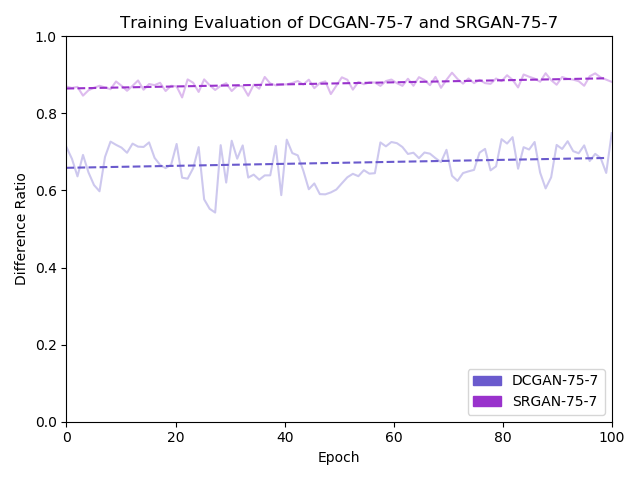
\includegraphics[width=8cm]{training_75-7.png}}
\centerline{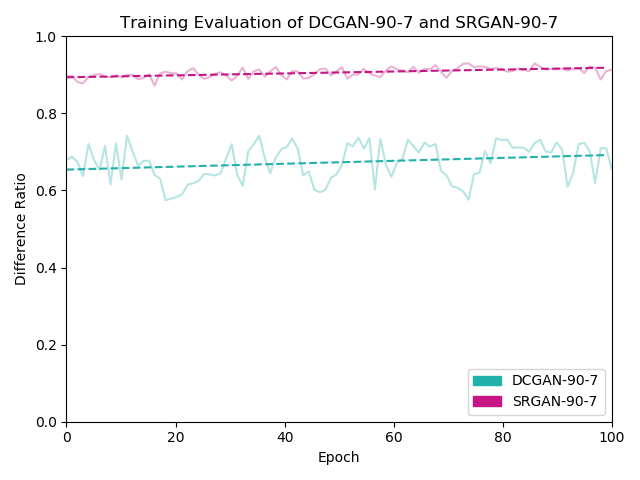
\includegraphics[width=8cm]{training_90-7.png}}
\centerline{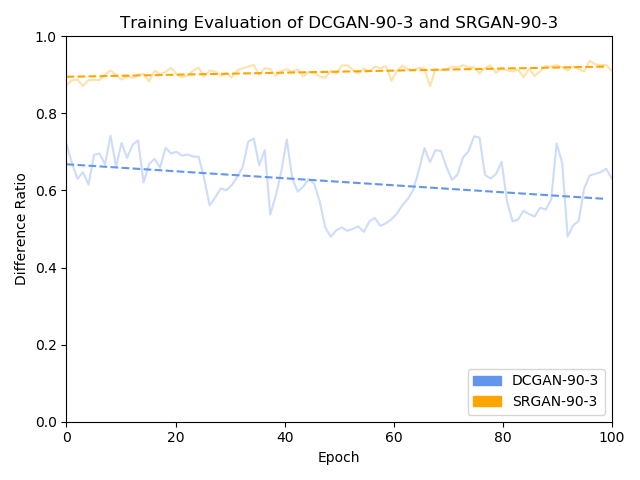
\includegraphics[width=8cm]{training_90-3.png}}
\caption{Model percentage enhancement of fake output to real source for all parameter values.}
\label{fig:training}
\end{figure}

%\begin{figure*}[tbp]
%\centerline{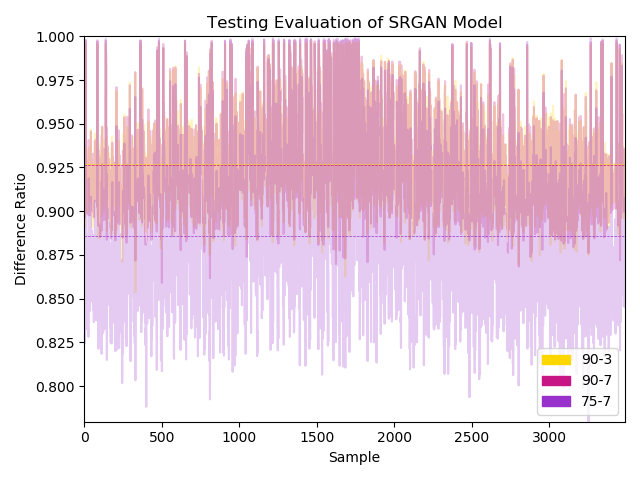
\includegraphics[width=0.75\textwidth]{testing_srgan_composite.png}}
%\caption{SRGAN percentage fake output is to real source for all parameter values.}
%\label{fig:srgan_composite}
%\end{figure*}

Since the value of enhancement for the DCGAN was not as well learned,
the only model evaluated with the testing set was the SRGAN.
Figure \ref{fig:srgan_testing_separate} shows the calculated enhancement for
all testing samples. The average enhancement for each distribution is drawn in
a horizontal dashed line. These averages are also recorded in Table \ref{tbl:enhancement}.

\begin{figure}[htbp]
\centerline{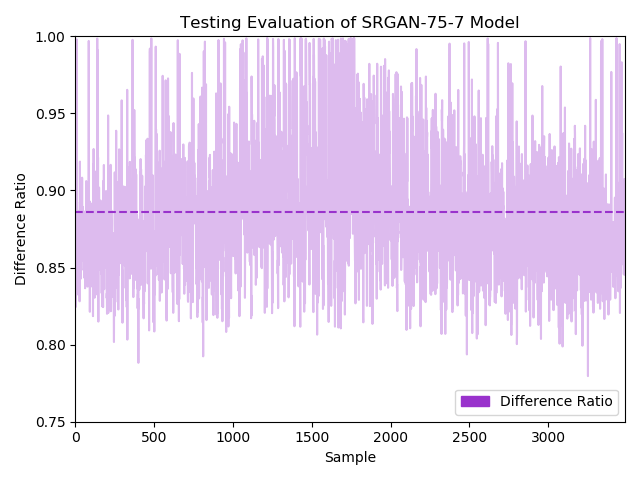
\includegraphics[width=8cm]{testing_srgan_75-7.png}}
\centerline{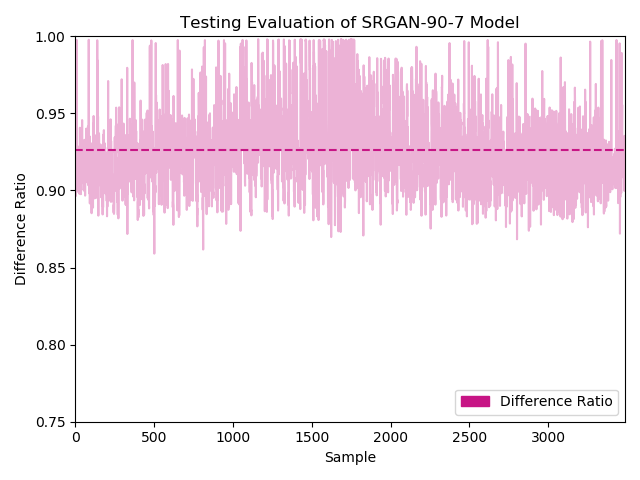
\includegraphics[width=8cm]{testing_srgan_90-7.png}}
\centerline{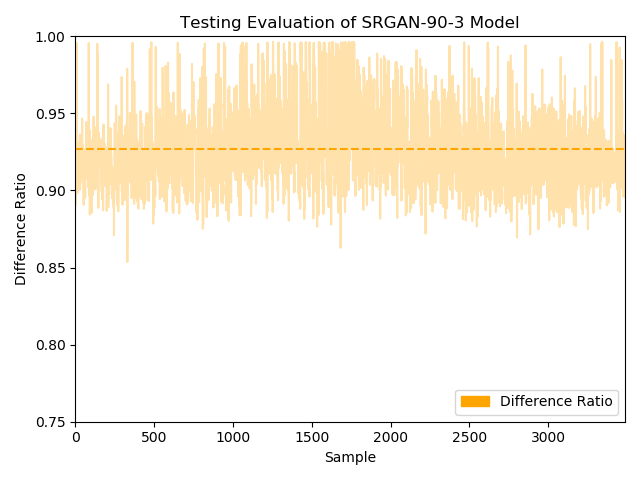
\includegraphics[width=8cm]{testing_srgan_90-3.png}}
\caption{SRGAN percentage fake output is to real source for all parameter values.}
\label{fig:srgan_testing_separate}
\end{figure}

\begin{table}[t]
\caption*{Average Enhancement}
\begin{centering}
\bgroup
\def\arraystretch{1.5}
\begin{tabular}{| m{0.14\textwidth} | m{0.09\textwidth} | m{0.09\textwidth}|} 
\hline
Parameters ($\alpha,\beta$) & DCGAN & SRGAN \\ 
\hline
\hline
$\alpha = 0.75$, $\beta = 7$ & 0.6523212 & 0.7694525 \\
\hline
$\alpha = 0.90$, $\beta = 7$ & 0.6563784 & 0.8579113 \\
\hline
$\alpha = 0.90$, $\beta = 3$ & 0.6040223 & 0.8365252 \\
\hline
\end{tabular}
\bigskip
\caption{Evaluation for the goodness of fit.}
\label{tbl:enhancement}
\egroup
\end{centering}
\end{table}

Average enhancement for the 75-7 SRGAN model on testing data was 0.8860892.
The 90-7 and 90-3 SRGAN models were closer together, with enhancements of
0.9263004 and 0.9270327, respectively.
These results clearly show the impact of noise when training the model.
Switching from $\beta = 3$ to $\beta = 7$ created an insignificant change
compared to the increase of $\alpha = 0.75$ to $\alpha = 0.90$.
Thus, noise more heavily impacted results than blur.
This effect is demonstrated by the samples shown in Figure \ref{fig:srgan_outputs};
the most distorted image is still close to the target, but not nearly as close as the
images with less noise.

\begin{figure}[htbp]
\centerline{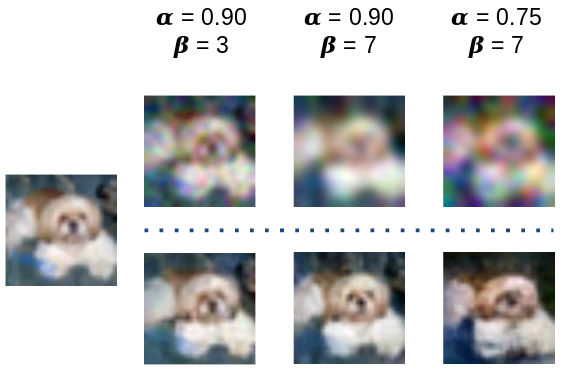
\includegraphics[width=8cm]{srgan_outputs.png}}
\caption{Example outputs from the test set for the SRGAN model.
The true image is shown on the left, while the generated images for each
set of parameters is shown below.}
\label{fig:srgan_outputs}
\end{figure}

\section{Future Work}
The next step for the project will be to complete the implementation for the
Sparse Attention (Transformer) architecture. It is expected that this architecture
will give better results than either of the DCGAN and SRGAN architectures.
The SRGAN architecture already achieved an average enhancement of up to 92\%
the quality of the target image.
We also plan to tweak the SRGAN model such that it uses
convolutional and convolutional-transpose layers in D and G, respectively.
The result should be a DCGAN version of the original SRGAN.
Comparing the results of the modified model to the original will provide
insight into how the layer changes affected the model's output.

Another study that will be performed is a variation of image degradation,
to test whether the trained models can learn how to enhance images with alterations
over the spectrum of parameter values.
This factor will be important for evaluating a model's
capabilities in general.

\section{Conclusion}
Image enhancement is a widely-studied problem, with new advancements in the field
being made each year.
In order to find the best model possible for enhancing low quality images,
we will evaluate several machine learning architectures.
Current tests show promise in the GAN architecture,
specifically the SRGAN model that was used for testing.
While the original DCGAN model faired poorly, it will be interesting to see the
impacts of modifying the layers of the SRGAN into a DCGAN-type architecture.
While results have yet to be collected from the Transformer,
the non-convolutional model will be an excellent comparison once completed.
The project will conclude with an extrapolation on future research
and the implications of our results on generalized image enhancement.

%\nocite{overview}

\bibliography{midterm}
\bibliographystyle{aaai}

\end{document}
